%% LaTeX2e class for student theses
%% sections/content.tex
%% 
%% Karlsruhe Institute of Technology
%% Institute for Program Structures and Data Organization
%% Chair for Software Design and Quality (SDQ)
%%
%% Dr.-Ing. Erik Burger
%% burger@kit.edu
%%
%% Version 1.1, 2014-11-21



\section{}




\chapter{Theoretical Framework}
\label{chap:chap_theo}

\newacronym{cfd}{CFD}{computational fluid dynamics}
\newacronym{smb}{SMB}{simulated moving bed chromatography}

In the first part of this chapter the fundamentals of magnetism are described. Section \ref{subsec:Quant_mag} gives an overview of the basic magnetic quantities while in section \ref{subsec:Mag_mat} the magnetic properties of materials are discussed. In Section \ref{sec:Mag_sep} the basic principles of and the forces acting in a magnetic separation process are explained. Furthermore the dimensioning of a Helmholtz coil is described in Section \ref{sec:Dim_helm_coil}.
In the second part of this chapter the fundamentals of \gls{cfd} are discussed (see Section ...). 

\section{Fundamentals of magnetism}
\label{sec:Fund_mag}
Magnetism is a physical phenomenon produced by the motion of electric charges, which results in attractive and repulsive forces between objects \cite{stevenson2010oxford}. Electric currents and the magnetic moments of elementary particles are at the origin of magnetic fields, which generate these forces. 

\subsection{Maxwell's Equations}
\label{subsec:Maxwell}
%%%%%%%%%Quellen einfügen%%%%%%%%%%%%%%%%%%%%%%%%%%%%%%%%%%%%%%%%%%% \cite{kallenbach2018elektromagnete}
The relationship between magnetic and electric fields as well as the relation of those fields to electrical charges and currents is described by  Maxwell’s equations. In combination with the Lorentz force law these equations describe all classical electromagnetic phenomena \cite{SWB-427138094} . The macroscopic Maxwell equations for general time-varying fields in the differential form are as follows: 

\begin{equation}
\label{eq:Faraday}
\centering
\nabla\times\boldsymbol{E} = -\frac{\partial\boldsymbol{B}}{\partial t}
\end{equation}

\begin{equation}
\label{eq:Ampere}
\centering
\nabla\times\boldsymbol{H} = \boldsymbol{J} + \frac{\partial\boldsymbol{D}}{\partial t}
\end{equation}

\begin{equation}
\label{eq:Gauss_elec}
\centering
\nabla\cdotp\boldsymbol{D} = \rho 
\end{equation}

\begin{equation}
\label{eq:Gauss_mag}
\centering
\nabla\cdotp\boldsymbol{B} = 0
\end{equation}

where the used fundamental electromagnetic quantities are the electric field intensity $\boldsymbol{E}$ in V/m, the magnetic flux density $\boldsymbol{B}$ in T, the magnetic field intensity $\boldsymbol{H}$ in A/m, the electric current density $\boldsymbol{J}$ in A/m\textsuperscript{2}, the electric flux density $\boldsymbol{D}$ in C/m\textsuperscript{2} and the electric charge density $\rho$ in C/m\textsuperscript{3}. Equation \ref{eq:Faraday}, also referred to as Faraday's law, describes how a time varying magnetic field induces a spatially varying electric field, while Equation \ref{eq:Ampere} (Ampere's law) states that magnetic fields are generated by either electric currents or time varying electric fields. Together they describe the propagation of electromagnetic waves. Equation \ref{eq:Gauss_elec} and \ref{eq:Gauss_mag} are called Gauss's law and Gauss's law of magnetism respectively. Equation \ref{eq:Gauss_elec} gives the effect of the charge density on the electric field. It states that the electric flux through any hypothetical closed surface is proportional to the net electric charge enclosed by this surface. Gauss's law of magnetism states that, contrary to electric charges, magnetic charges, also called magnetic monopoles, do not exist and that $\boldsymbol{B}$ is always a solenoidal vector field. Instead a magnetic field is induced by magnetic dipoles. Through the relationship of $\boldsymbol{B}$ and $\boldsymbol{H}$ (see Equation \ref{eq:B_vac}) the divergence of the magnetic field intensity is also zero \cite{monk2003finite} \cite{kallenbach2018elektromagnete}.
The combination of Gauss' and Ampere's law results in the continuity equation (see Equation \ref{eq:Konti_Mag}) which specifies the conservation of charge. It states that the net quantity of charges is always conserved \cite{monk2003finite}.   

\begin{equation}
\label{eq:Konti_Mag}
\centering
\nabla\cdotp\boldsymbol{J} = -\frac{\partial\rho}{\partial t}
\end{equation}

For static fields, i.e. no variation of the field quantities with time, the Equations \ref{eq:Faraday}, \ref{eq:Ampere} and \ref{eq:Konti_Mag} are reduced to:

\begin{equation}
\label{eq:Faraday_stat}
\centering
\nabla\times\boldsymbol{E} = 0
\end{equation}

\begin{equation}
\label{eq:Ampere_stat}
\centering
\nabla\times\boldsymbol{H} = \boldsymbol{J} 
\end{equation}

\begin{equation}
\label{eq:Konti_Mag_stat}
\centering
\nabla\cdotp\boldsymbol{J} = 0
\end{equation}

\subsection{Constitutive relations}
\label{subsec:const_rel}

In order to apply Maxwell's macroscopic equations they must be augmented with two constitutive relations. The constitutive relations describe the relationship between $\boldsymbol{D}$ and $\boldsymbol{E}$ as well as between $\boldsymbol{B}$ and $\boldsymbol{H}$ depending on the macroscopic properties of the medium. The constitutive relations in empty space can be written as

\begin{equation}
\label{eq:disp_const_rel}
\centering
\boldsymbol{D} = \varepsilon_{0}\boldsymbol{E} 
\end{equation}

\begin{equation}
\label{eq:B_vac}
\centering
\boldsymbol{B} = \mu_{0}\boldsymbol{H}
\end{equation}

with the vacuum permittivity $\varepsilon_{0}$ with a value of 8.854$\cdotp$10\textsuperscript{-12}\,F/m and the vacuum permeability $\mu_{0}$ with a value of 4$\pi\cdotp$10\textsuperscript{-7} H/m \cite{monk2003finite}. For linear materials the relationship between $\boldsymbol{B}$ and $\boldsymbol{H}$ is   

\begin{equation}
\label{eq:B_tot}
\centering
\boldsymbol{B} = \mu_{0}\mu_{r}\boldsymbol{H}
\end{equation}

where $\mu_{r}$ indicates the relative permeability of the medium. The relative permeability is a measure of the permeability of a material relative to that of an vacuum (see Equation \ref{eq:mu_r}). Materials with $\mu_{r}$ larger than one are called paramagnetic, while materials with a value of $\mu_{r}$ less than one are referred to as diamagnetic. In contrast ferromagnetic materials exhibit a hysteresis function (see Section \ref{subsec:Mag_mat}).  

\begin{equation}
\label{eq:mu_r}
\centering
\mu_{r} = \frac{\mu}{\mu_{0}}
\end{equation}

The magnetic flux density is also influenced by the magnetization $\boldsymbol{M}$ of the material as shown below: 

\begin{equation}
\label{eq:Mag}
\centering
\boldsymbol{B} = \mu_{0}(\boldsymbol{H} + \boldsymbol{M})
\end{equation}

For linear materials there is a directly proportional relationship between the magnetization and the magnetic field intensity with the magnetic suceptibility $\chi$.  

\begin{equation}
\label{eq:chi}
\centering
\boldsymbol{M} = \chi\boldsymbol{H}
\end{equation}

Materials with positive values of $\chi$ are paramagnetic, were as materials with negative values of $\chi$ are called diamagnetic. For ferro- and ferrimagnetic materials $\chi$ is dependent on the previous magnetization of the medium. The magnetic suceptibility is also related to the relative permeability (see Equation \ref{eq:chi_2}).

\begin{equation}
\label{eq:chi_2}
\centering
\chi = \mu_{r}-1
\end{equation}

For some materials there is no linear relationship between $\boldsymbol{B}$ and $\boldsymbol{H}$ as shown in Equation \ref{eq:nonlin_B}.

\begin{equation}
\label{eq:nonlin_B}
\centering
\boldsymbol{B} = f(\vert\boldsymbol{H}\vert)
\end{equation}


\subsection{Magnetic properties of materials}
\label{subsec:Mag_mat}
Figure of permeability curves

\section{Fundamentals of magnetic separation}
\label{sec:Mag_sep}

\subsection{Basic principles}
\label{subsec:bas_princ}

\subsection{Magnetic particle accumulation on single wires}
\label{subsec:single_wire}

\section{Dimensioning of a Helmholtz coil}
\label{sec:Dim_helm_coil}

\section{Simulated moving bed chromatography}
\label{sec:smb}

\chapter{Materials and Methodology}
\label{chap:chap_mat}
\newacronym{pva}{PVA}{polyvinyl alcohol}
\newacronym{pmma}{PMMA}{polymethyl methacrylate}
\newacronym{ptfe}{PTFE}{polytetrafluorethylen}
\newacronym{fplc}{FPLC}{Fast Protein Liquide Chromatography}
\newacronym{esem}{ESEM}{Environmental scanning electron microscope}
\newacronym{agm}{AGM}{Alternating Gradient Magnetometer}

In the first part of this chapter the model setup and implementation using the simulation software COMSOL Multiphysics\textsuperscript{\textregistered}, thereafter referred to as COMSOL, is described.\\
Section \ref{sec:Exp_setup} gives an overview of the experimental setup and execution as well as the analytical and evaluation methods used.  


\section{Model setup/Development}
\label{sec:Model_setup}
The objective of this thesis was the design and implementation of (to establish) an in silico model simulating the retention of magnetic nanoparticles flowing through a magnetizable packed bed. Furthermore parameter studies for various conditions were conducted. In the following the simulation setup including geometry, mesh, boundary conditions and solvers is described.    

\section{Experimental setup}
\label{sec:Exp_setup}
For the validation of the simulation results and a proof of principle of the operational concept several experimental runs were designed. In order to evaluate the retention of a magnetic nanoparticle suspension within a magnetizable packed bed a chromatographic system was used (see Section \ref{subsec:chrom_sys}). The nanoparticle suspension is characterized in Section \ref{subsec:Mag_nanoparticles} and the matrix materials in Section \ref{subsec:Matrix_mat}. Furthermore an overview of the conducted experiments is given in Section \ref{subsec:Exp_Pro}. In Section \ref{subsec:ana_met} the analytical methods and in Section \ref{subsec:Eval} the evaluation methods are discussed.    


\subsection{Magnetic nanoparticle suspension}
\label{subsec:Mag_nanoparticles}
The experiments were conducted with two different types of magnetic nanoparticles. For the experiments in Section \ref{subsec:Exp_Pro} a nanoparticle suspension from Chemagen was used. The magnetic nanoparticles from Chemagen consist of a core of magnetite coated with \gls{pva}. A stock solution with a concentration of 73\,g/l was used. In order to minimize aggregation, the stock solution was put into an ultrasonic bath for 20 minutes before use. Then the stock solution was diluted 1:100 with 20\,mM sodium phosphate buffer with a pH of 6.5 and filterd through a filter with a pore size of 450\,nm. 
In addition,  plain nanomag\textsuperscript{\textregistered}-D-spio particles from micromod with mean diameters of 20\,nm and 100\,nm were utilized for the experiments. The micormod nanoparticles are composed of iron oxid domains coated by an unmodified dextran surface. The stock solution with a concentration of 25\,g/l was also diluted 1:100 with a 20\,mM phosphate buffer. In additon a 1:1 mixture of the two nanoparticle sizes was used. In contrast to the Chemagen nanoparticles, the micromod particles required no additional ultrasonic treatment and filtration in order to remove aggregates.     

\subsection{Matrix material}
\label{subsec:Matrix_mat}
For the packed bed three different matrix materials were evaluated. In Table \ref{table:mat_material} the two magnetizable materials and their corresponding composition are listed. The concentration ranges for the TruForm particles are due to protected confidentiality. %check this! ask for real composition    

\begin{table}[H]
\centering
\caption{Matrix materials and their composition}
\label{table:mat_material}
\begin{tabular}{llllllll}\hline
\multirow{2}{*}{name} & \multirow{2}{*}{charge/lot} & \multirow{2}{*}{producer} & \multicolumn{5}{c}{composition in \%}  \\
& & & Fe & C & Cr & Ni & Mo \\
\hline\hline
SRA-150 & W140401E & H.C. Stark & 83.95 & 0.16 & 12.5  & & \\
TruForm\textsuperscript{TM} 316-3 & 15 & Praxair & 50-75 & & 5-20 &5-20& 1-5\\
\hline
\end{tabular}
\end{table}

The matrix material SRA-150 was already used in preceding experiments by \cite{AndreMaster}. In order to achieve a narrow particle-size distribution the SRA-150 particles were sieved with a mesh size of 25\,\textmu m and 20\,\textmu m respectively. In addition the matrix material TruForm 316-3 was chosen due to its spherical structure and material composition. 
As a negative control \gls{pmma} particles from microParticles GmbH were used. 

\subsection{Column packing}
\label{subsec:col_pack}
As chromatographic column a Omnifit\textsuperscript{\textregistered} BenchMark\textsuperscript{TM} Microbore chromatography column (Omnifit Labware, Diba Industries, Danbury, USA) was used. The borosilicate glass column has a column length of 10\,mm, a column inside diameter of 3\,mm and a total volume capacity of 0.7\,ml. On both sides of the column endpieces with pre-assembled frits were used to hold back the matrix material. For the experiments with \gls{pmma} and SRA-150 \gls{ptfe} frits with a pore size of 25\,\textmu m were used. In addition punched out polycarbonate filters with a pore size of 2\,\textmu m and an O-ring were added to the inlet and outlet of the column. For the experiments with the TruForm 316-3 matrix material \gls{ptfe} frits with a pore size of 5\,\textmu m were used, no additional filters were necessary. \\   
For the column packing a slurry consisting of the matrix material and either ultra-pure water for \gls{pmma} or a 20\,\% Ethanol suspension for SRA-150 and TruForm 316-3 was used. Ethanol was used in order to simplify the packing of the column due to the reduced surface tension. To remove impurities and achieve a narrower particle size distribution the \gls{pmma} matrix material was first mixed with the solvent and left to settle for several minutes. After sedimentation the supernatant was removed and replaced by fresh solvent. This procedure was repeated till the supernatant was a clear fluid. For the other two matrix materials instead of sedimentation a magnet was held to the outside of the falcon to seperate the magnetizable particles from the supernatant.\\   
A CETONI neMESYS syringe pump (CETONI GmbH, Korbussen, Germany), controlled by a QmixElements software, was connected to bottom of the column via a tube (see Figure \ref{fig:Packing_Setup_Column}). With this set-up a negative pressure was generated within the column into which the matrix material slurry is drawn from the column inlet. The slurry was added to the column inlet by a pipette. Once the column was completely filled, the syringe pump was disconnected and the endpiece with the corresponding frit or filter was placed on top of the column. Then the packed bed within the column was compressed with the help of an \gls{fplc}-system (described in Section \ref{subsec:chrom_sys}) to eliminate possible cavities. Afterwards the column was again connected to the syring pump and the resulting void at the top filled with new matrix material. This procedure was repeated until no further compression of the matrix material could be observed. The column and the syringe pump are shown in Figure \ref{fig:Packing_Setup_Column}.
%%%%%%%%%%%%%%%%%%%%Include Figure of setup and column%%%%%%%%%%%%%%%%%%%%%%%%%%%%%%%%%%%%%%%%%%%%%%%%%%%%%%%%%%%%%%%%%%%%%%%%%%%%%%%%%%%%%%%%%%%%%%%%%%%%%%%%%%%%%%

\begin{figure}[h]
		%\centering
          \begin{subfigure}{0.49\textwidth}
                  \flushleft
                  \scalebox{0.12}{\includegraphics{figures/Column_Packing_All_numbers.pdf}}
                  %\caption{Packing setup}\label{fig:Packing}
          \end{subfigure}\hfill
        \begin{subfigure}{0.49\textwidth}
                \flushright
                \scalebox{0.0545}{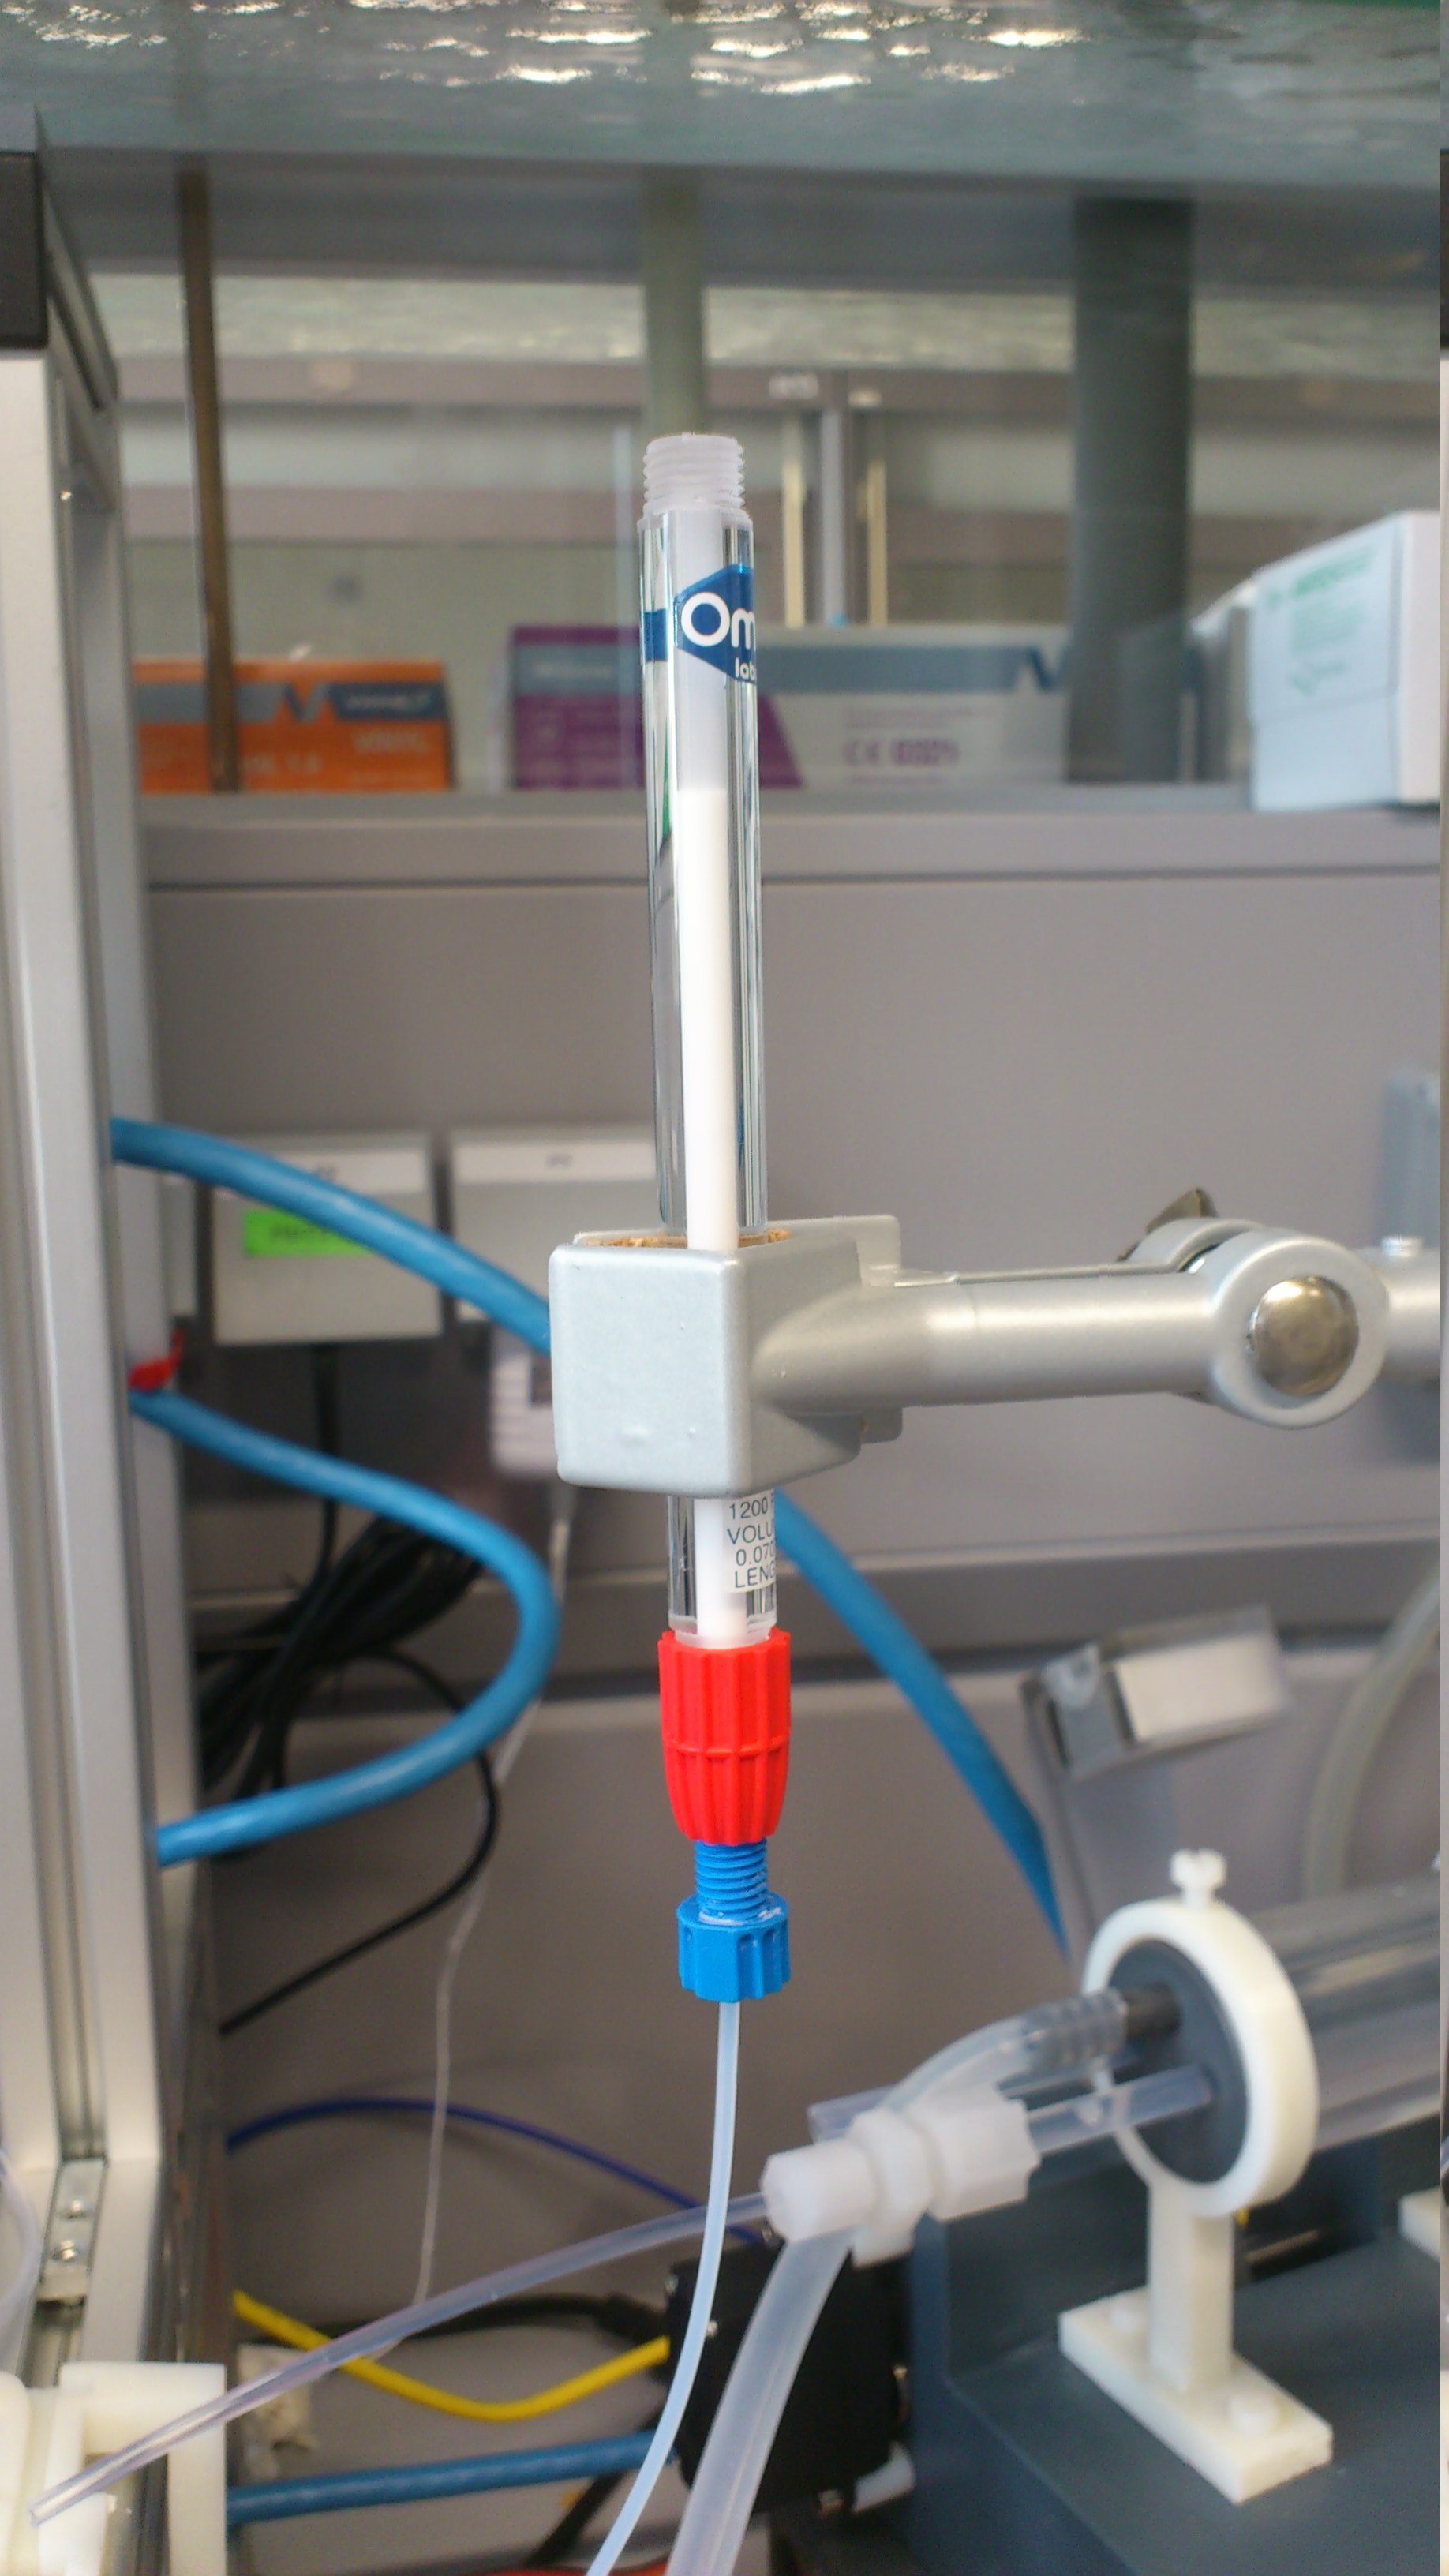
\includegraphics{figures/Column_Packing_Column.jpg}}
                %\caption{Column}\label{fig:Column}
        \end{subfigure}
        \\
        
        \caption[Column packing setup]{Column packing setup; left side: CETONI neMESYS control station (1), column (2) and syring pump (3); right side: Column packed with \gls{pmma} matrix material }
        \label{fig:Packing_Setup_Column}
  \end{figure}  




% \begin{figure}[H]
% \centering
% 
% \scalebox{0.30}{\includegraphics{Bioreactor_real.png}}
% \caption{Photobioreactor with 37 light cylinders for the cultivation of microalgae
% \label{fig: Bioreactor_real}
% }
% \end{figure} 
% 
% \begin{figure}[h]
% 		\centering
%           \begin{subfigure}{0.49\textwidth}
%                   \flushleft
%                   \scalebox{0.30}{\includegraphics{Bioreactor_Geometry.png}}
%                   \caption{Lateral view of the photobioreactor}\label{fig:Bioreactor_Geometry}
%           \end{subfigure}
%         \begin{subfigure}{0.49\textwidth}
%                 \flushright
%                 \scalebox{0.32}{\includegraphics{Bioreactor_cross_section.png}}
%                 \caption{Cross section of the photobioreactor}\label{fig:Bioreactor_cross_section}
%         \end{subfigure}
%         \\
%         
%         \caption{Structure of the photobioreactor with 37 light cylinders}
%         \label{fig:Bioreactor}
%   \end{figure}  


\subsection{Chromatographic system}
\label{subsec:chrom_sys}
For the compression of the packed bed within the column and the execution of the retention experiments an Äkta purifier \gls{fplc}-system from GE Healthcare (Buckinghamshire, England) was used. For all connections tubings with an inner diameter of 0.25\,mm (PEEK tubings blue, GE Healtcare Bio-Sciences AB, Uppsala, Sweden) were used to achieve high resolution peaks. The samples were injected via a sample loop with a total volume of 100\,\textmu m. The experiments were conducted with ultra-pure water as solvent and a constant flow rate. An inline UV flow cell was used to continuously measure the absorbance of the liquid at a wavelength of 280 nm and to transmit the data to the computer. A conductivity flow cell was used to measure the conductivity of the passing solution. For further analysis the samples were collected by a fraction collector. The regulation of the \gls{fplc}-system and the analysis of the transmitted data was realized by the software Unicorn. The experimental setup is shown in Figure \ref{fig:  }.
%%%%%%%%%%%%%%%Include Figure of ÄKta and Fraction collector%%%%%%%%%%%%%%%%%%%%%

\subsubsection{Chromatographic system with a Helmholtz coil}
\label{subsubsec:helm_coil}
For all experiments a Helmholtz coil was used to create a stable homogeneous magnetic field around the column. The Helmholtz coil consists of an assembly of four coils with the distance D between each other. The whole length of the four coils was based on the length of the column. The other calculated dimensions of the Helmholtz coil can be found in Table \ref{table:Helmholtz_coil}. The Helmholtz coil was constructed so that for a current of 2\,A a magnetic field of 14\,mT was created. The coil was also designed to be used in an ultrasonic bath. The technical drawing for the construction of the used Helmholtz coil is shown in Figure \ref{fig:Helmholtz_coil}\\  
The Helmholtz coil was included in the chromatographic system as shown in Figure \ref{fig: ???}. The coil was connected to a power amplifier (19 Z/500, FG Elektronik) to increase the electrical signal and therefore the magnetic field within the coil. The square wave signals were generated by a function generator (Rigol DG1022, RIGOL Technologies Inc., Beijng, China). The adjustment of the magnetic flux density was achieved by the regulation of the electric current measured with a digital multimeter(MY64, Mastech Group LLC., CA, USA).   

\begin{table}[H]
\centering
\caption[Dimensions of the Helmholtz coil]{Calculated dimensions of the Helmholtz coil}
\label{table:Helmholtz_coil}
\begin{tabular}{ll}\hline
Parameter &  Value \\
\hline\hline
 number of turns in each coil n & 300 \\
 filling factor F & 0.73\\
 diameter of copper wire $d_{D}$ & 0.70\,mm\\
 coil depth & 10\,cm\\
 distance between coils D & 3.3\,cm \\
 inner radius $R_{i}$ & 3.0\,cm\\ 
 outer radius $R_{a}$ & 4.58\,cm\\
 mean/average radius $R_{m}$ & 3.79\,cm\\
 \hline
\end{tabular}
\end{table}


\begin{figure}[H]
		\centering
          \begin{subfigure}{0.49\textwidth}
                  \flushleft
                  \scalebox{0.40}{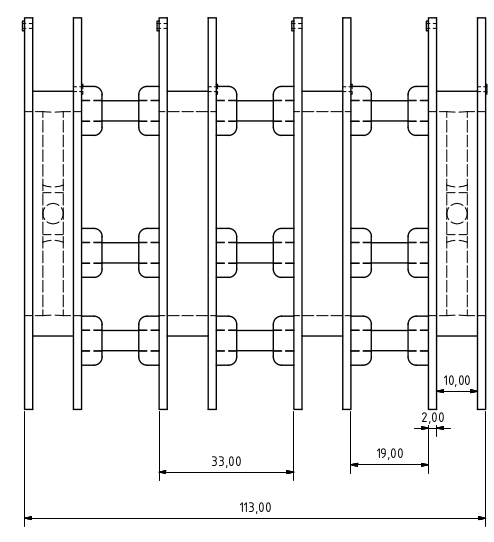
\includegraphics{figures/Helmholtz_Coil_Full.png}}
                  \caption{Side view of the Helmholtz coil}\label{fig:Coil_Full}
          \end{subfigure}
        \begin{subfigure}{0.49\textwidth}
                \flushright
                \scalebox{0.5}{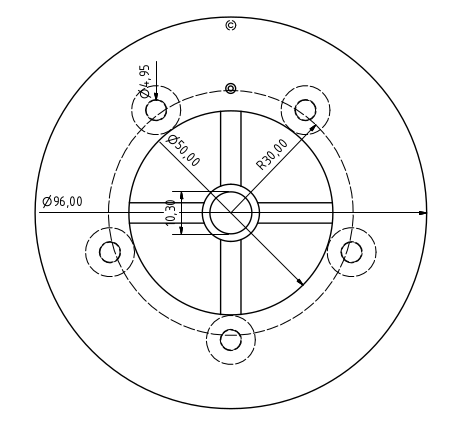
\includegraphics{figures/Helmholtz_Coil_Top.png}}
                \caption{Top view of the Helmholtz coil}\label{fig:Coil_Top}
        \end{subfigure}
        \\
        
        \caption[Technical drawing of the Helmholtz coil]{Technical drawing of the Helmholtz coil with length specifications in mm }
        \label{fig:Helmholtz_coil}
  \end{figure}  

\subsection{Experimental procedures}
\label{subsec:Exp_Pro}
All experiments were programmed and regulated using the control software Unicorn 5.20 (GE Healthcare Life Sciences). Before each injection the column was washed with 2\,ml of ultra-pure water to remove remaining nanoparticles from the previous injection. To achieve comparability and reproducibility all experiments were conducted with the same method, except for the fractionation and saturation experiments ,for which a separate method was created. All experiments were done in triple determination. \\
Before each experiment series the quality of the column packing was controlled. For this purpose a one percent acetone solution was injected and the asymmetry of the  resulting UV peak analyzed. For a packing with \gls{pmma} an asymmetry between 1 and 2 and for a packing with the TruForm particles an asymmetry between 1 and 1.5 was considered tolerable. For deviating asymmetry values the column was emptied and repacked. After each experiment series the column was demagnetized with the help of a degaussing coil (Entmagnetisierer EM-60, MAGNET-PHYSIK Dr. Steingroever GmbH, Cologne, Germany). Afterwards the column was washed until no significant change in the UV signal was perceived anymore. To clean the filters of the column and reduce the back pressure a change between up- and down-flow was applied while washing when necessary. Once a pressure of 50\,bar was reached the filters were replaced. The blocked filters were regenerated by storing them for 24 hours in oxcalic acid with a concentration of 250\,g/l on a stirrer plate with the lowest heating level.

\subsubsection{Flow rate optimization}
\label{subsubsec:Flow_rate}
In a first step the flow rate was optimized for each matrix material. For this purpose flow rates of 0.1\,ml/min, 0.2\,ml/min and 0.5\,ml/min were tested. The nanoparticle suspension was injected with a volume of 100\,\textmu l and the above mentioned method (see Section \ref{subsec:Exp_Pro}) run with the corresponding flow rates. The resulting UV peaks were analyzed for their asymmetry and reproducibility. Also the comparability with the results from \cite{AndreMaster} was taken into consideration.  

\subsubsection{Retention of magnetic nanoparticle suspension}
\label{subsubsec:Ret_nanopart_method}
The main objective of this experiments was to asses the retention of the magnetic nanoparticles through a magnetized packed bed. The magnetization of the packed bed was achieved by the Helmholtz coil described in Section \ref{subsubsec:helm_coil}. The homogeneous magnetic field within the coil was created by a power amplifier connected to a function generator, which generated an alternating current with a square wave signal. The power amplifier was used to change the electric signal and thereby vary the magnetic flux density. For all experiments a flow rate of 0.5\,ml/min and magnetic flux densities between 0\,mT and 17\,mT were used. \\
The magnetic field could be influenced by the variation of the frequency, duty cycle and amplitude. A constant magnetic field was produced by setting the high and low state to the closest values possible. The smallest difference achievable with the used function generator was 4\,mV. Therefore a high level value of 400\,mV and a low level value of 396\,mV was used to approximate a direct current (see Figure \ref{fig:waveform}). To investigate the impact of an alternating magnetic field the low level was set to -\,400\,mV wereas the high level stayed at 400\,mV. To simulate a magnetic field being turned on and off a low level value of 0\,mV was chosen. For the matrix material \gls{pmma} all described variations were applied with the frequencies 100\,mHz and 1000\,mHz . For the matrix material Stark and TruFrom only the constant and on/off fields with frequencies of 100\,mHz, 500\,mHz and 1000\,mHz were tested. The duty cycle, the ratio of the high period to the total period of the square wave, was set to 50\,\% for all experiments. An exception was an experiment with the TruForm particles were the off phase was reduced to 20\,\%.

\begin{figure}[h]
\centering

\scalebox{0.60}{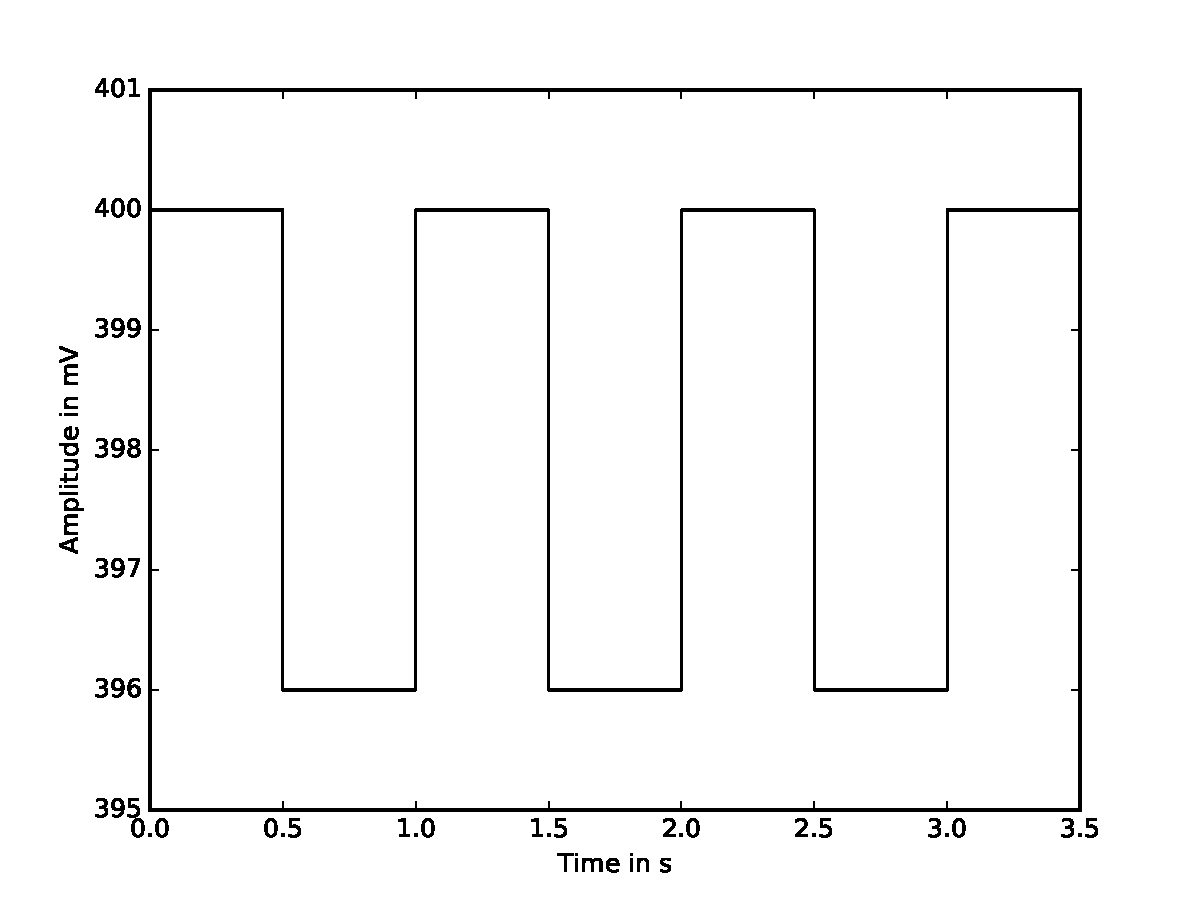
\includegraphics{figures/waveform.pdf}}
\caption[Example of a square wave signal]{Example of a square wave signal used for the generation of a constant magnetic field with a frequency of 1\,Hz, a high level of 400\,mV and a low level of 396\,mV
\label{fig:waveform}
}
\end{figure}


In addition saturation experiments were conducted with the TruForm material. For those experiments the column was first washed with 1\,ml and no magnetic field, next the sample solution was injected and the constant magnetic field was turned on. The magnetic field was held till the column was washed with 2\,ml. The cycle was repeated till no further change in the UV peak could be observed. The experiment was conducted twice, once with an used and once with a new filter. A magnetic flux density of 17\,mT was used for the saturation experiments.\\
In order to evaluate the influence of the nanoparticle concentration on the retention behaviour, Chemagen nanoparticel suspension was diluted 1:100, 1:150 and 1:200. The dilutions were tested with TruForm matrix material and a constant magnetic field. The micromod nanoparticle suspensions were also only used for experiments with the TruForm matrix material and a constant magnetic field.\\
For further analysis the third peak of each triple determination was fractionated and collected in 1.5\,ml Eppendorf tubes. A Unicorn method was written to start the fractionation as soon as an increase in the UV signal was detected. As fraction volume 200\,\textmu l was chosen. The fractionation was stopped as soon as the UV signal sank below 0.1\,mAu. 
 

%%%%%%%%%Tabelle mit Parametern ?%%%%%%%%%%%%%%%%%%%%%%%%%%%%%%%%%%%%%%%%%%%%%%%%%
 

\subsection{Analytical methods}
\label{subsec:ana_met}
 For the characterization of the matrix materials and the nanoparticle suspensions several different analytical methods were used. The particle size distribution was determined either by dynamic light scattering, light micrsocope or under the \gls{esem} described in Sections \ref{subsubsec:part_dist_meas}, \ref{subsubsec:light_mic} and \ref{subsubsec:ESEM}. The method for the determination of the magnetic properties is described in Section \ref{subsubsec:Mag_char}. For characterization of the magnetic field within the Helmholtz coil a Hall effect sensor was used (see Section \ref{subsubsec:Hall_eff}).   
 
 
\subsubsection{Measurement of particle size distributions}
\label{subsubsec:part_dist_meas}
For the determination of the particle size distribution two different measurement devices were used. The matrix materials were analyzed with an CIS 100-S particle sizer (Galai, Migdal Haemek, Israel). The measurement system combines two analytical techniques, namely laser obstruction time analysis and dynamic image analysis to analyze both the size distribution and shape factors of the sample. For the laser obstruction time measurement a helium-neon laser with a wavelength of 600\,nm rotates with a constant frequency and interacts with particles in the sample solution. Each scanned particle temporarily blocks the path of the laser beam to the corresponding photo diode, which registers the time of transition. The obstruction time in combination with the frequency is then related to the particle diameter \cite{neis1997particle}. Additionally dynamic image analysis is used to determine the particle shape parameters. With this combination spherical and non-spherical particles in a range between 0.1\,\textmu m to 3,600\,\textmu m can be measured. For each sample a three-fold determination was conducted, with a length of 60\,s for each measurement cycle. In addition the reproducibility of the measurement was verified by the measurement software. As sample preparation a spatula tip of the matrix material was mixed with 2\,ml of ultra-pure water. Of this suspension 1500\,\textmu l were filled into a cuvette. If necessary the sample was further diluted with ultra-pure water. During the measurement period the suspension was continuously mixed with a pipette (Eppendortf Research \textsuperscript{\textregistered} plus (blue), Eppendorf AG, Hamburg, Germany) to ensure homogeneity. \\
\\
For the determination of the particle size distributions of the magnetic nanoparticle suspensions and the collected nanoparticle fractions (see Section \ref{subsubsec:Ret_nanopart_method}) a Zetasizer Nano ZSP (Malvern Instruments, Malvern, England) was used. The nanoparticle stock suspensions were diluted 1:100 in ultra-pure water, while for the fractions no further dilution was necessary. The Chemagen nanoparticle solution was measured in filtered and unfiltered form (see Section \ref{subsec:Mag_nanoparticles}), whereas the micromod particles were not filtered at all. For each measurement 50\,\textmu l of the sample was pipetted into a quarz cuvette and put into the Zetasizer. For all samples a triple determination was conducted. The size measurement was performed by dynamic light scattering. Particles scatter the light from a helium-neon laser with a wavelength of 633\,nm creating a fluctuation in the detected scattering intensity over time. This fluctuation is due to the Brownian motion, which leads to diffusion of particles at a speed related to their size and temperature. From the intensity changes a correlation function is generated from which the diffusion coefficient is deducted. The particle size distribution is then calculated with the Stokes-Einstein equation \cite{berne2000dynamic}. Particle sizes could be measured in the range of 0.3\,nm to 10\,\textmu m \cite{Zetasizer}. For the evaluation only particles in the nanometer size range were considered. In order to reduce the influence of contaminations, either leaked matrix material or dust, within the samples, all particles with a size of over 1\,\textmu m were not included in the size distributions.

\subsubsection{Environmental scanning electron microscope}
\label{subsubsec:ESEM}
The particle shape, size and surface properties were characterized with an \gls{esem} (XL 30-FEG, Philips, Amsterdam, Netherlands). \gls{esem} is a procedure in which uncoated samples can be examined with an electron beam. The samples to be analyzed were placed within the sample chamber. Then a vacuum was applied reaching pressures between 130\,Pa and 1300\,Pa. An electron beam is focused on the sample which leads to the ejection of secondary electrons from the sample surface. These secondary electrons are then accelerated towards the electric field of an detector. The detected signal is converted into an image of the sample. With this method it is possible to magnify the samples by a factor of 50 up to 5100 \cite{danilatos1993introduction}.     
\gls{esem} measurements were used for the characterization of the TruForm matrix material. As sample preparation a defined quantity of the matrix material was put on a sample holder. No further sample preparation was needed.

\subsubsection{Light microscope}
\label{subsubsec:light_mic}
The characterization of the \gls{pmma} matrix material was conducted with the help of a VHX-5000 digital microscope system (Keyence, Osaka, Japan). A 500 frames per second camera captures image data with different focus positions and generates high resolution images on an attached monitor. By variation of the shutter speed the resolution and contrast are further increased. In addition the optimal wavelength to generate clear images is automatically selected \cite{VHX5000}. For the measurement the matrix material was suspended in ultra-pure water. A few drops of the suspension were placed on a slide and put onto the object stage. The magnification was slowly increased until a high resolution image was aquired. By measuring the distance from two neighbouring pixel on the screen dimension measurements were possible. With this method the mean diameter of the measured matrix particles was determined.    


\subsubsection{Concentration determination of the nanoparticle suspension}
\label{subsubsec:Conc_MF}
For the determination of the Chemagen nanoparticle concentration 200\,\textmu l of the particle suspension was filled into an HPLC vial. All measurements were conducted in triple determination. Before filling the empty weight of the vials was determined with a MC5 microbalance (Sartorius, Göttingen, Germany). The vials were dried for 24 hours at \SI{60}{\celsius} in a drying cabinet (drying cabinet ULE 500, Memmert GmbH, Schwabach, Germany). The vials were allowed to cool in a desiccator for 20 minutes and then weighed again. From the difference between the current and the empty weight the mass of the magnetic nanoparticles could be calculated. With the calculated mass and the used suspension volume the concentration could be determined.  


\subsubsection{Magnetization determination of the matrix materials and nanoparticle suspension}
\label{subsubsec:Mag_char}
The characterization of the magnetic properties of the matrix materials was performed with an \gls{agm} (Micromag 2900, Princeton Measurments Corp, Princeton, USA). As sample preparation a defined amount of matrix material was given onto a strip of adhesive tape and hermetically sealed with another piece of tape. The sample was then placed onto a cantilevered rod including a piezoelectric element, magnetized by a dc field and overlaid by an oscillating magnetic field gradient. Through the  oscillating magnetic field gradient the sample experiences an alternating force  which is proportional to the magnitude of the field gradient and the magnetic moment of the sample. This force deflects the sample rod within the magnetic field which leads to a voltage output of the piezoelectric element. With a variation of the alternating magnetic field strength the voltage signals can be converted into a magnetization curve \cite{flanders1988alternating}. The magnetization within the magnetization curve was normalized with the mass of the used sample. Before the actual measurements, the \gls{agm} was calibrated with a nickel standard. From the hysteresis loop the magnetic properties of the materials could be extracted. On all samples a threefold determination was performed.    

\subsubsection{Analysis of the magnetic flux density}
\label{subsubsec:Hall_eff}
The magnetic flux density within the Helmholtz coil was measured with a Hall effect sensor (FH 31/4, MAGNET-PHYSIK Dr. Steingroever GmbH, Cologne, Germany). The Hall effect sensor consists of a thin rectangular p-type semiconductor material on which a constant current is applied. When the sensor is placed in a magnetic field perpendicular to the current the electrons are deflected towars one edge of the sensor. The result is a potential difference that develops between the upper and lower edge of the conductor which is referred to as the Hall voltage. The Hall voltage is proportional to the applied current and the magnetic flux density \cite{svoboda2004magnetic}.\\%%%%%V=-(I*B)/(e*rho*t) 
The magnetic flux density of the Helmholtz coil was measured for different currents in six different positions along the symmetry axis. The resulting flux density was then compared to the calculated values for the Helmholtz coil (see Section \ref{subsubsec:helm_coil}). 


\subsection{Evaluation methods}
\label{subsec:Eval}
For the evaluation of both, the particle size distribution and the retention experiments, evaluation routines were written in python. Wherever possible the same evaluation methods as in \cite{AndreMaster} were applied to ensure comparability. 

\subsubsection{Graphical evaluation}
\label{subsubsec:Graph_eval}
In order to compare the results from the particle size distribution measurements, the D-values D10, D50 and D90 were determined. D50 is defined as the diameter where half of the particles are smaller than this value. Likewise 10\,\% of the population lie below the value from D10 and 90\,\% below the value of D90 \cite{merkus2009particle}. The cumulative distribution is  approximated by a least squares polynomial fit, where the solution minimizes the squared error E (see Equation \ref{eq:polyfit_er}) for the equations shown in \ref{eq:polyfit_eq}.  

\begin{equation}
\label{eq:polyfit_er}
\centering
E = \sum_{j=0}^{k}\vert p(x_{j})-y_{j}\vert^{2}
\end{equation}

\begin{equation}
\label{eq:polyfit_eq}
\centering
\begin{split}
x[0]^{n}p[0] + ... + x[0]p[n-1] + p[n] = y[0] \\
x[1]^{n}p[0] + ... + x[1]p[n-1] + p[n] = y[1]  \\
... \\ 
x[k]^{n}p[0] + ... + x[k]p[n-1] + p[n] = y[k]
\end{split}
\end{equation}

Where $p$ represents the polynomial coefficients, $n$ the degree of the polynomial, $y$ the y-coordinates and $x$ the x-coordinates of the sample points. The coefficient matrix of the coefficient $p$ is called Vandermonde matrix \cite{bjorck1970solution}. With this fit the D-values were calculated. 
%%%%%%%%%%%%%%%%Add Number distribution%%%%%%%%%%%%%%%%%%%%%%%%%%%%%%%%%%%%%

\subsubsection{Mathematical evaluation}
\label{subsubsec:Math_eval}
For the evaluation of the retention experiments with the magnetic nanoparticle suspensions the UV signal from the \gls{fplc}-system was used. The influence of the magnetic field was determined by a comparison of the UV peak area and retention with the retention and area of a control peak with no magnetic field applied. The area of the peak (see Equation \ref{eq:area}) provides information about the particles bound in the packed bed at a certain magnetic field strength.    

\begin{equation}
\label{eq:area}
\centering
area = \sum_{j=1}^{N}[(x_{i+1}-x_{i})(\frac{y_{i+1}+y_{i}}{2})]
\end{equation}

The first term on the right side of Equation \ref{eq:area} depicts an infinitely small interval of the volume which has flown through the column in ml. While the second term describes the average of the UV signal in mAU within the limits of x. The results were normalized by dividing the area of a peak with an applied magnetic field by the area of a standard peak without the influence of ante magnetic field. \\

%%%%%%%%%Check this find better description%%%%%%%%%%%%%%%%%%%%%%%%%%%%%%%%

The equations for the calculation of the retention of the nanoparticles are shown in the following: 

\begin{equation}
\label{eq:ret_sum}
\centering
k = k_{s} = \sum_{j=1}^{N}[(x_{i+1}-x_{i})(\frac{y_{i+1}+y_{i}}{2})(\frac{x_{i+1}+x_{i}}{2})]
\end{equation}

\begin{equation}
\label{eq:ret_comp}
\centering
retention = \frac{k}{k_{s}}
\end{equation}

In order to evaluate the influence of the retention the average of volume $(x_{i+1}+x_{i})/2$ within the infinitely small interval of $x_{i+1}-x_{i}$ was added to the area. The retention $k$ of a field under magentic influence was also normalized by the division with the retention $k_{s}$ of a standard peak.   

%%%%%%%%%%%%%%%%%%%%%%%%%%%%%%%%%%%%%%%%%%%%%%%%%%
%%%%%%%%%%%%%%%%%%%%%%%%%%%%%%%%%%%%%%%%%%%%%%%%%%
%%%%%%%%%%%%%%%%%Results%%%%%%%%%%%%%%%%%%%%%%%%%%
%%%%%%%%%%%%%%%%%%%%%%%%%%%%%%%%%%%%%%%%%%%%%%%%%%
%%%%%%%%%%%%%%%%%%%%%%%%%%%%%%%%%%%%%%%%%%%%%%%%%%


\chapter{Results and Discussion}8
\label{chap:chap_res}

\section{Simulation results}
\section{Experimental results}

